\begin{minipage}{0.75\linewidth}
\begin{figure}[h]
    \centering
    \begin{adjustbox}{max width=1.0\linewidth, keepaspectratio}
        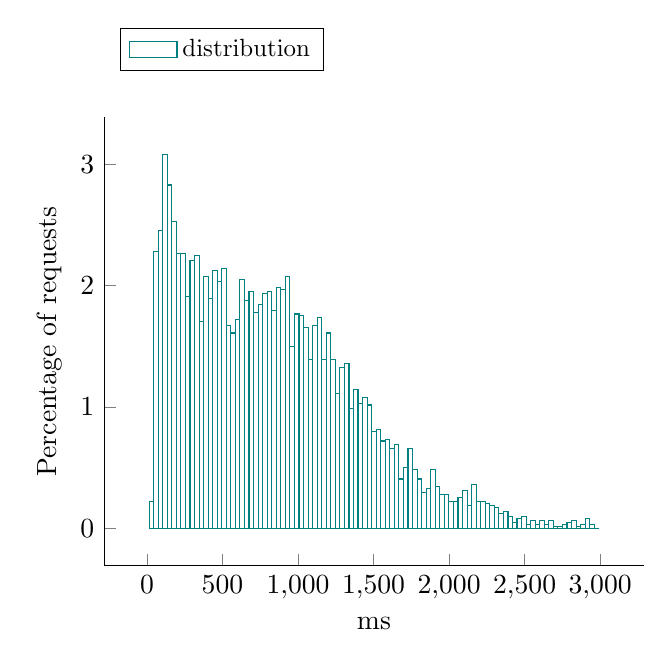
\begin{tikzpicture}
            \begin{axis}[ylabel = Percentage of requests, 
xlabel = ms, 
legend style = {nodes={scale=0.9, transform shape}, at={(0.03,1.2)}, anchor=north west, draw=black, fill=white, align=left, legend columns=3},
area style, mark size = 0pt,
 cycle list name = exotic,
  axis lines* = left]
		\addplot +[ybar interval] coordinates {
			 (14, 0.21875)
			 (44.07, 2.28125)
			 (74.14, 2.45312)
			 (104.21, 3.07812)
			 (134.28, 2.82812)
			 (164.35, 2.53125)
			 (194.42, 2.26562)
			 (224.49, 2.26562)
			 (254.56, 1.90625)
			 (284.63, 2.20312)
			 (314.7, 2.25)
			 (344.77, 1.70313)
			 (374.84, 2.07812)
			 (404.91, 1.89062)
			 (434.98, 2.125)
			 (465.05, 2.03125)
			 (495.12, 2.14062)
			 (525.19, 1.67188)
			 (555.26, 1.60938)
			 (585.33, 1.71875)
			 (615.4, 2.04688)
			 (645.47, 1.875)
			 (675.54, 1.95312)
			 (705.61, 1.78125)
			 (735.68, 1.84375)
			 (765.75, 1.9375)
			 (795.82, 1.95312)
			 (825.89, 1.79687)
			 (855.96, 1.98438)
			 (886.03, 1.96875)
			 (916.1, 2.07812)
			 (946.17, 1.5)
			 (976.24, 1.76562)
			 (1006.31, 1.75)
			 (1036.38, 1.65625)
			 (1066.45, 1.39062)
			 (1096.52, 1.67188)
			 (1126.59, 1.73438)
			 (1156.66, 1.39062)
			 (1186.73, 1.60938)
			 (1216.8, 1.39062)
			 (1246.87, 1.10938)
			 (1276.94, 1.32812)
			 (1307.01, 1.35938)
			 (1337.08, 0.984375)
			 (1367.15, 1.14062)
			 (1397.22, 1.03125)
			 (1427.29, 1.07812)
			 (1457.36, 1.01562)
			 (1487.43, 0.796875)
			 (1517.5, 0.8125)
			 (1547.57, 0.71875)
			 (1577.64, 0.734375)
			 (1607.71, 0.65625)
			 (1637.78, 0.6875)
			 (1667.85, 0.40625)
			 (1697.92, 0.5)
			 (1727.99, 0.65625)
			 (1758.06, 0.484375)
			 (1788.13, 0.40625)
			 (1818.2, 0.296875)
			 (1848.27, 0.328125)
			 (1878.34, 0.484375)
			 (1908.41, 0.34375)
			 (1938.48, 0.28125)
			 (1968.55, 0.28125)
			 (1998.62, 0.21875)
			 (2028.69, 0.21875)
			 (2058.76, 0.25)
			 (2088.83, 0.3125)
			 (2118.9, 0.1875)
			 (2148.97, 0.359375)
			 (2179.04, 0.21875)
			 (2209.11, 0.21875)
			 (2239.18, 0.203125)
			 (2269.25, 0.1875)
			 (2299.32, 0.171875)
			 (2329.39, 0.125)
			 (2359.46, 0.140625)
			 (2389.53, 0.09375)
			 (2419.6, 0.046875)
			 (2449.67, 0.078125)
			 (2479.74, 0.09375)
			 (2509.81, 0.03125)
			 (2539.88, 0.0625)
			 (2569.95, 0.03125)
			 (2600.02, 0.0625)
			 (2630.09, 0.03125)
			 (2660.16, 0.0625)
			 (2690.23, 0.015625)
			 (2720.3, 0.015625)
			 (2750.37, 0.03125)
			 (2780.44, 0.046875)
			 (2810.51, 0.0625)
			 (2840.58, 0.015625)
			 (2870.65, 0.03125)
			 (2900.72, 0.078125)
			 (2930.79, 0.03125)
			 (2960.86, 0)
			 (2990.93, 0)
		};
\addlegendentry{distribution};
           \end{axis}
      \end{tikzpicture}
  \end{adjustbox}
  \caption{Response time distribution - req = ReadTimeline-0}
\end{figure}
\end{minipage}\hfill\begin{minipage}{0.18\linewidth}
\begin{table}[h]
\begin{tabular}{|cc|}
\hline
\textbf{} & \textbf{ms}\\ \hline
 \Xhline{0.005\arrayrulewidth}
min & 14\\
 \Xhline{0.005\arrayrulewidth}
max & 3021\\
 \Xhline{0.005\arrayrulewidth}
mean & 825\\
 \Xhline{0.005\arrayrulewidth}
std & 562\\
\hline
\hline
 \Xhline{0.005\arrayrulewidth}
25th & 358\\
 \Xhline{0.005\arrayrulewidth}
50th & 754\\
 \Xhline{0.005\arrayrulewidth}
75th & 1179\\
 \Xhline{0.005\arrayrulewidth}
80th & 1288\\
 \Xhline{0.005\arrayrulewidth}
85th & 1418\\
 \Xhline{0.005\arrayrulewidth}
90th & 1592\\
 \Xhline{0.005\arrayrulewidth}
95th & 1887\\
 \Xhline{0.005\arrayrulewidth}
99th & 2374\\
\hline
\end{tabular}
\caption{Response time}
\end{table}
\end{minipage}\hfill